\part{Data Preparation}
    The selected data range spans from 2000 to 2016, which is consistent across multiple datasets. However, an exception exists for the happiness dataset, which includes data exclusively from 2005. The shared fields, serving as integration keys, are 'year' and 'country' for the tables.
    \\
    \\
    To facilitate validation and seamless integration, a supplementary dataset will be generated to address missing country values.
    \\
    \\
    To enhance clarity in describing the process, each dataset will be individually addressed for “Select the data”, “Clean the data”, and “Construct the data”, ensuring a more comprehensive understanding of the procedures involved. The final integration and formatting will be explain for all the datasets. All the data imputations will be done over the merged final table.
    \\
    \\
    It's crucial to note that through joins and outer joins, the datasets other than the one furnishing obesity information will initially aim to align all records for every year and country present in the obesity dataset.


    \section{\dsMissingCountries}

        \subsection{Select the data}
            By utilizing the previously identified missing countries from each dataset (\figurename~\ref{fig:du-missing-countries-per-datasets-head-20}), a new dataset is constructed. This dataset includes the names of the missing countries and is then augmented with the actual corresponding names from the respective country's dataset. This approach facilitates a seamless merge through inner joins with each dataset, effectively ensuring the absence of missing data during integration with the other datasets.
            \\
            \\
            The table below illustrates the identified relationships between the missing countries and the corresponding datasets.
            \\
            \\

        \subsection{Construct the data}

            Manually, the names of the missing countries are located and substituted within a table featuring two columns: "country" and "replacement".
            \\
            \\
            This dataset will be used in the preparation process to make sure that the data integration will be properly done.

            In figure \figurename~\ref{fig:dp-missing-countries-replacements} each missing country has the replacement.
            \begin{figure}[H]
                \centering
                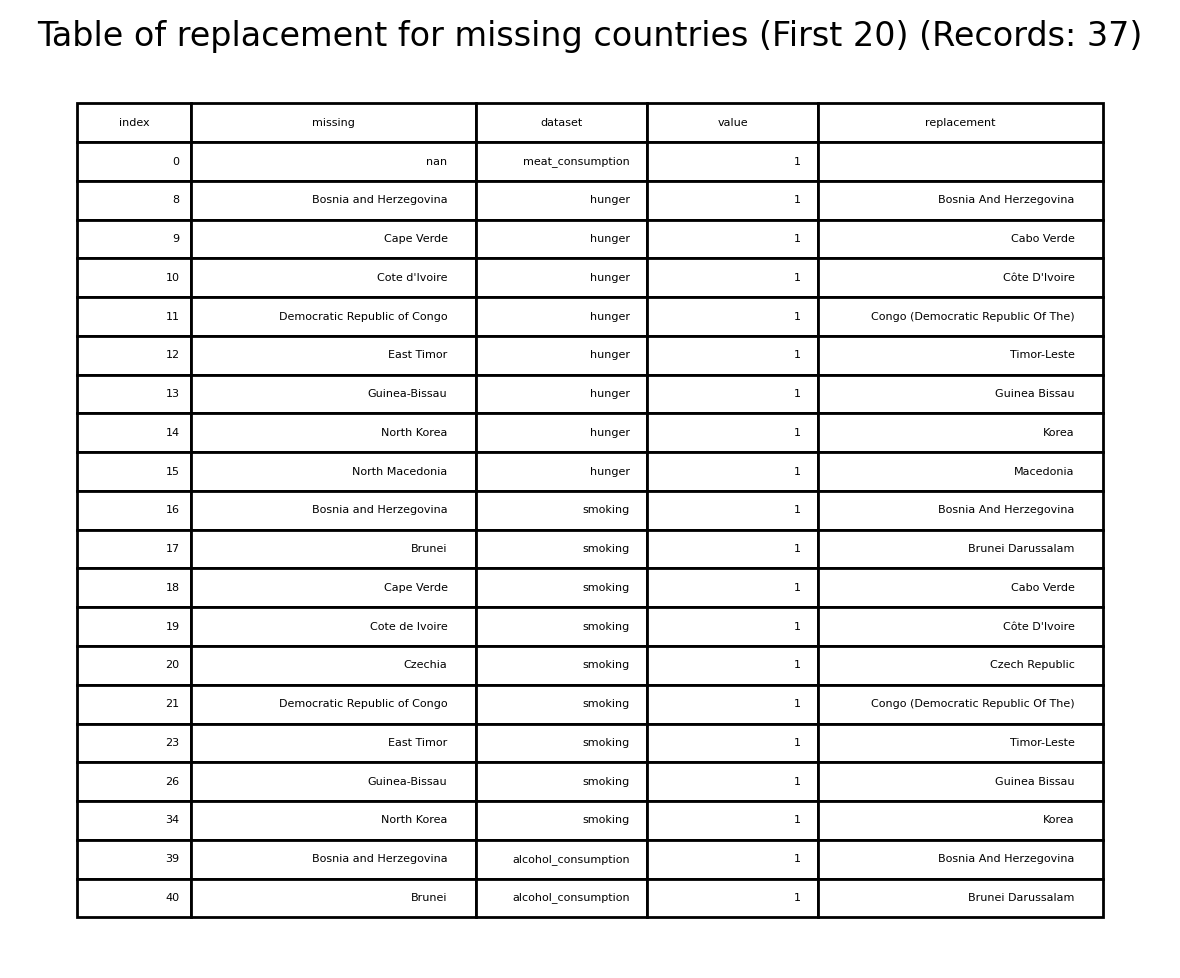
\includegraphics[scale=1]{images/dp_missing_countries_replacement}
                \caption{Dataset with the replacements for the missing countries in the other datasets.}
                \label{fig:dp-missing-countries-replacements}
            \end{figure}

            \subsubsection{Python Code for Replacing Missing Country Names}

                The following Python code snippet is used to map alternative country names to a standard form:

                \begin{verbatim}
missing_replacement = [
            ('Bosnia and Herzegovina', 'Bosnia And Herzegovina'),
            ('Czechia', 'Czech Republic'),
            ('North Macedonia', 'Macedonia'),
            ('Guinea-Bissau', 'Guinea Bissau'),
            ('Cape Verde', 'Cabo Verde'),
            ('East Timor', 'Timor-Leste'),
            ('North Korea', 'Korea'),
            ('Democratic Republic of Congo', 'Congo (Democratic Republic Of The)'),
            ('Brunei', 'Brunei Darussalam'),
            ('Viet Nam', 'Vietnam'),
            ('Hong Kong S.A.R. of China', 'Hong Kong'),
            ("Lao People's Democratic Republic", 'Laos'),
            ('United States of America', 'United States'),
            ('Democratic Republic of the Congo', 'Congo (Democratic Republic Of The)'),
            ('Congo (Kinshasa)', 'Congo'),
            ('Syrian Arab Republic', 'Syria'),
            ('United Kingdom of Great Britain and Northern Ireland', 'United Kingdom'),
            ('Bolivia (Plurinational State of)', 'Bolivia'),
            ('Ethiopia (former)', 'Ethiopia'),
            ('State of Palestine', 'Palestine'),
            ('Taiwan Province of China', 'Taiwan'),
            ('Turkiye', 'Turkey'),
            ('Türkiye', 'Turkey'),
            ("Democratic People's Republic of Korea", 'Korea'),
            ('United Republic of Tanzania', 'Tanzania'),
            ('Iran (Islamic Republic of)', 'Iran'),
            ('Republic of Moldova', 'Moldova'),
            ('Venezuela (Bolivarian Republic of)', 'Venezuela'),
            ('Russian Federation', 'Russia'),
            ('Micronesia (country)', 'Micronesia (Federated States of)'),
            ('Republic of Korea', 'Korea'),
            ("Cote de Ivoire", "Côte D'Ivoire"),
            ("Cote d'Ivoire", "Côte D'Ivoire"),
            ("Côte d'Ivoire", "Côte D'Ivoire"),
            ('Ivory Coast', "Côte D'Ivoire"),
        ]
                \end{verbatim}

        \subsection{Imputing the missing countries by joins}

            The dataset of missing countries will be used for completing the countries that are missing in the dataset. This process is explained here, to avoid repeating it across all the dataset, will be quite similar.
            \\
            \\
            Each dataset will be joined to missing countries by a left outer join.
            \\
            \\
            For every non-missing record in the "missing dataset" segment earmarked for replacement, it signifies that the corresponding entry must be corrected. Consequently, replacement occurs to rectify inaccuracies. This procedure is iteratively executed across all the other datasets.


    \section{\dsIntegratedDataset}

        \subsection{Handling Missing Countries}

            The initial step in the data preparation involved handling missing country names across the different datasets. A reference table was created, which contained mappings of alternative country names to a standardized name. This table was used to replace missing or differently written country names across all datasets, ensuring uniformity.

        \subsection{Dataset Merging}

            After the missing country names were standardized, all datasets were joined on two key attributes: the standardized country name and the year. This facilitated the merging of all disparate datasets into a single comprehensive table.

        \subsection{Column Renaming and Deletion}

            During the merging process, column names were standardized to ensure consistency. In the same step, columns that were not relevant to the modeling process were identified and removed, thus reducing the dimensionality of the dataset and streamlining it for analysis.

            By executing these steps, we were able to create a clean, organized, and unified dataset that is ready for further analysis and model building.

        \subsection{Cleaning the data}

            \subsubsection{Imputations: Deleting rows without important features}
                In addition to the above-mentioned data preparation steps, rows lacking sufficient information in essential columns were removed \figurename~\ref{fig:dp-removed-without-important-features}. Specifically, rows were inspected for missing values in key features essential for analysis and modeling. Such rows were deemed not useful, as the absence of these important variables would adversely impact the robustness and reliability of any subsequent analysis or predictive models. Therefore, to maintain data quality and integrity, these incomplete rows were eliminated from the dataset.
                \begin{figure}[H]
                        \centering
                        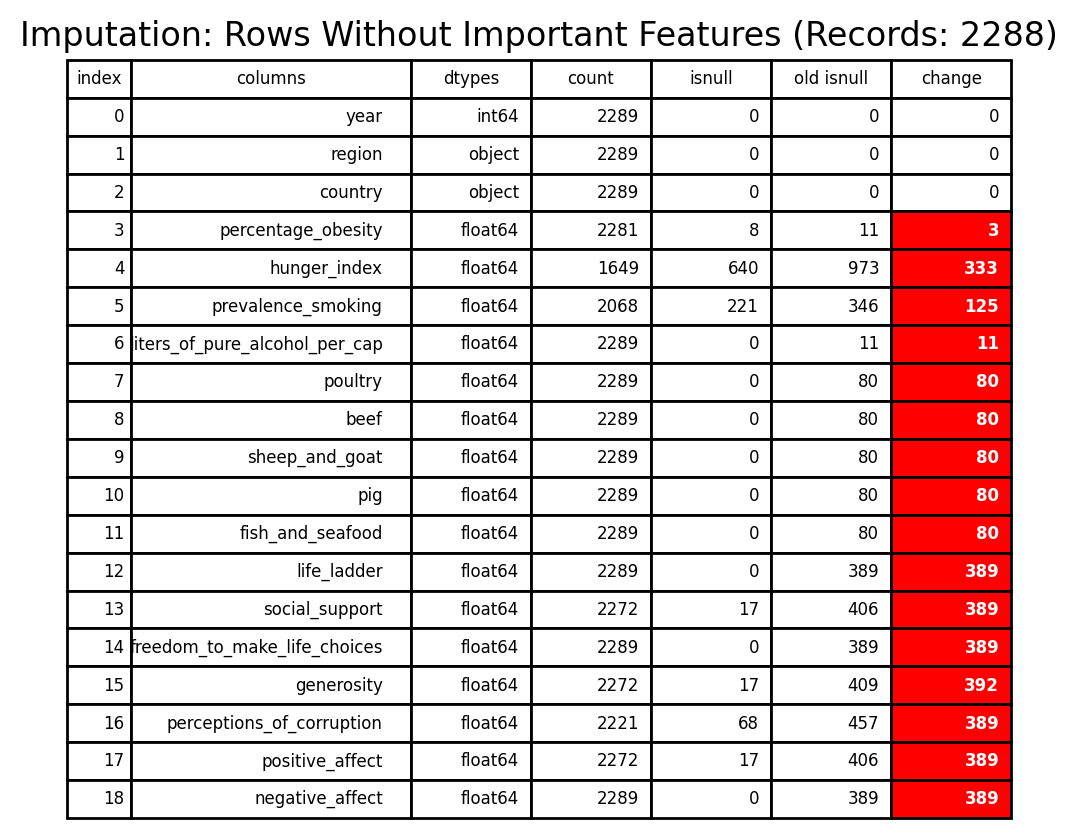
\includegraphics[scale=1]{images/dp_imput_impor_feat}
                        \caption{After the imputation done by deleting rows without important features.}
                        \label{fig:dp-removed-without-important-features}
                \end{figure}

            \subsubsection{Imputations: Countries that does not eat pig}
                The countries that does not have any record for pig are countries that does not consume that product. In this case the imputation will be 0
                \begin{figure}[H]
                        \centering
                        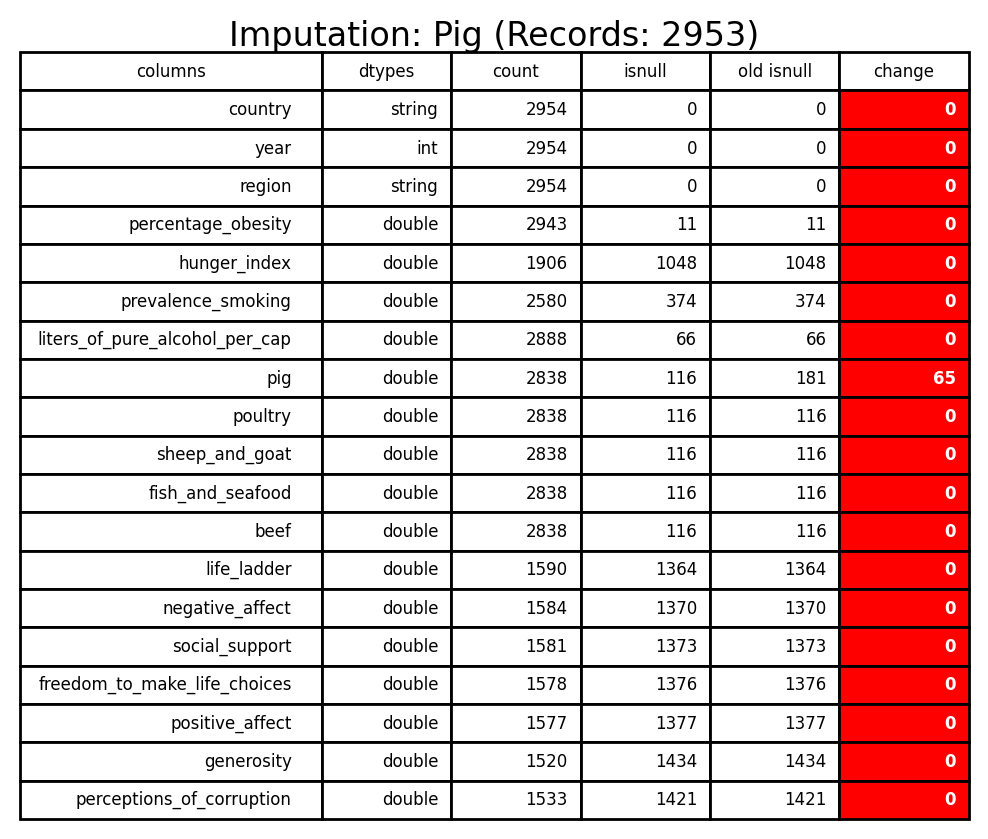
\includegraphics[scale=1]{images/dp_imput_pig}
                        \caption{Imputation for pig predicting with random forest.}
                        \label{fig:dp-imput-pig}
                \end{figure}

            \subsubsection{Imputations: By Group Country Year}

                For imputing the missing values in the following columns, we followed a similar strategy. Specifically, we used a grouped imputation method based on both the year and country.
                In this method, for each missing value within a given year-country group, the nearest available value was identified and then used to fill the missing data point. This approach ensures that the imputed value is the closest match to the missing data, providing a more accurate representation that respects the temporal and geographical context of the dataset.

                This imputation significantly reduced the number of missing values.


                Each imputation table provides insights into the imputation process for a specific column in the dataset. These tables display several critical pieces of information, outlined as follows:

                \begin{itemize}
                        \item \textbf{columns:} The column names of the dataset.
                        \item \textbf{dtypes:} Data types of each column.
                        \item \textbf{count:} The number of non-null entries in each column after imputation.
                        \item \textbf{isnull:} The number of null or missing entries in each column after imputation.
                        \item \textbf{old isnull:} The number of null or missing entries in each column before imputation.
                        \item \textbf{change:} The net change in the number (in red color) of missing entries as a result of the imputation. This is calculated as (\textit{old isnull} - \textit{isnull}).
                \end{itemize}

                For example, in the imputation table for the \texttt{liters\_of\_pure\_alcohol\_per\_capita} column, the \textit{change} value is 2038. This indicates that 2038 missing values were successfully imputed, reducing the \textit{isnull} count from 2049 to 11. This column-specific view allows us to evaluate the effectiveness of the imputation process for each attribute separately.

                The imputation tables serve as a quality assurance tool, helping us ensure that the dataset is as robust and complete as possible before proceeding to further stages of the analysis.

                \begin{figure}[H]
                        \centering
                        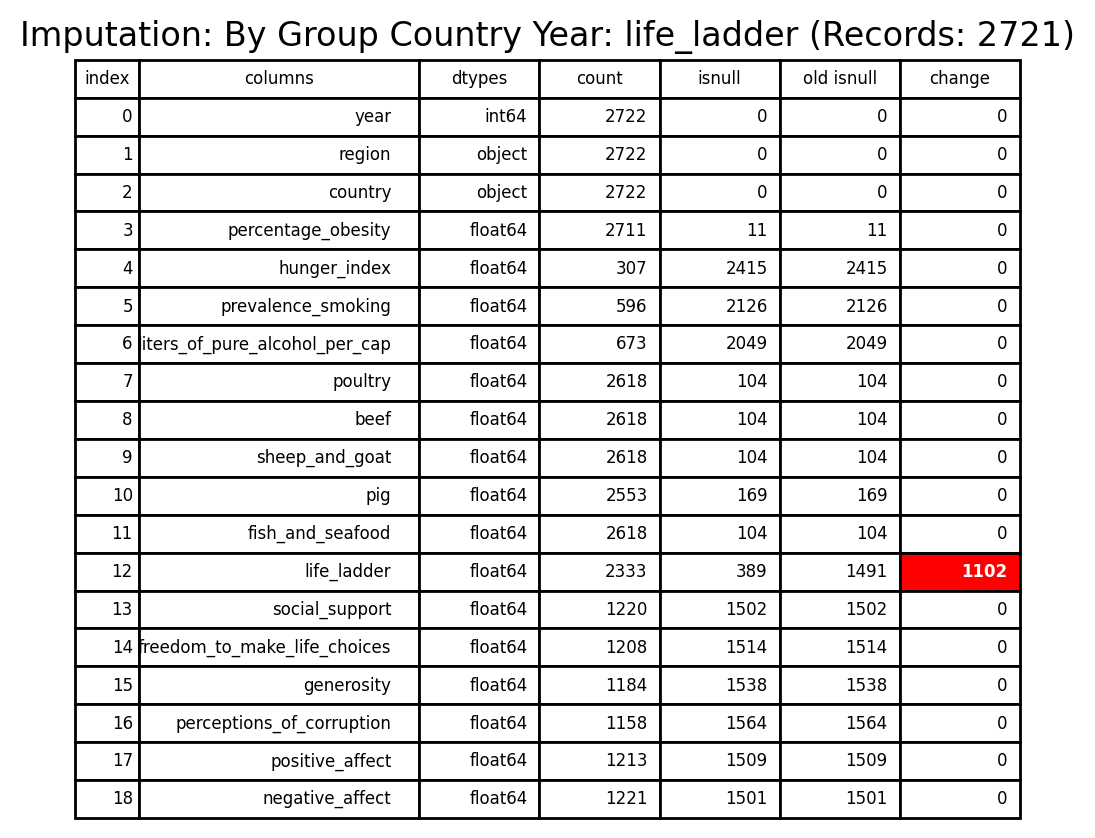
\includegraphics[scale=1]{images/dp_imputation_c_y_life_ladder}
                        \caption{Imputation for life\_ladder grouped by country year.}
                        \label{fig:dp-impute-group-country-life-ladder}
                \end{figure}

                \begin{figure}[H]
                        \centering
                        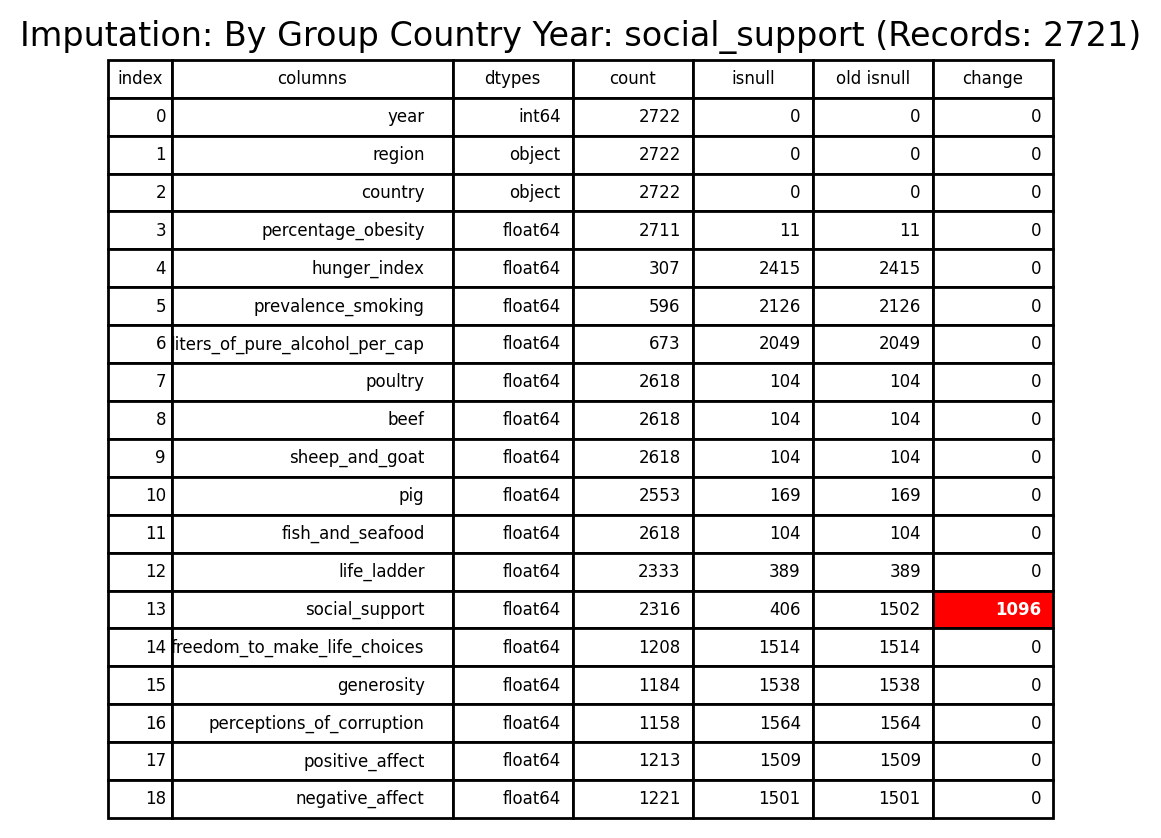
\includegraphics[scale=1]{images/dp_imputation_c_y_social_support}
                        \caption{Imputation for social\_support grouped by country year.}
                        \label{fig:dp-impute-group-country-social-support}
                \end{figure}

                \begin{figure}[H]
                        \centering
                        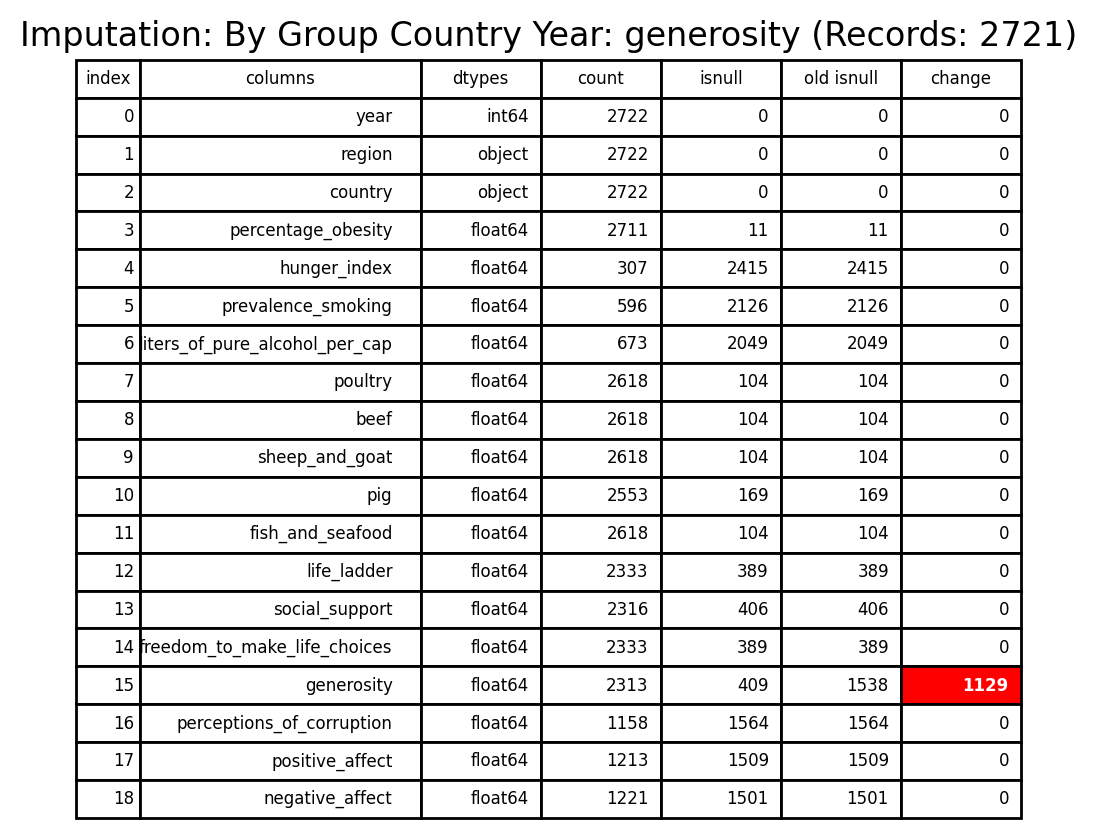
\includegraphics[scale=1]{images/dp_imputation_c_y_generosity}
                        \caption{Imputation for generosity grouped by country year.}
                        \label{fig:dp-impute-group-country-generosity}
                \end{figure}

                \begin{figure}[H]
                        \centering
                        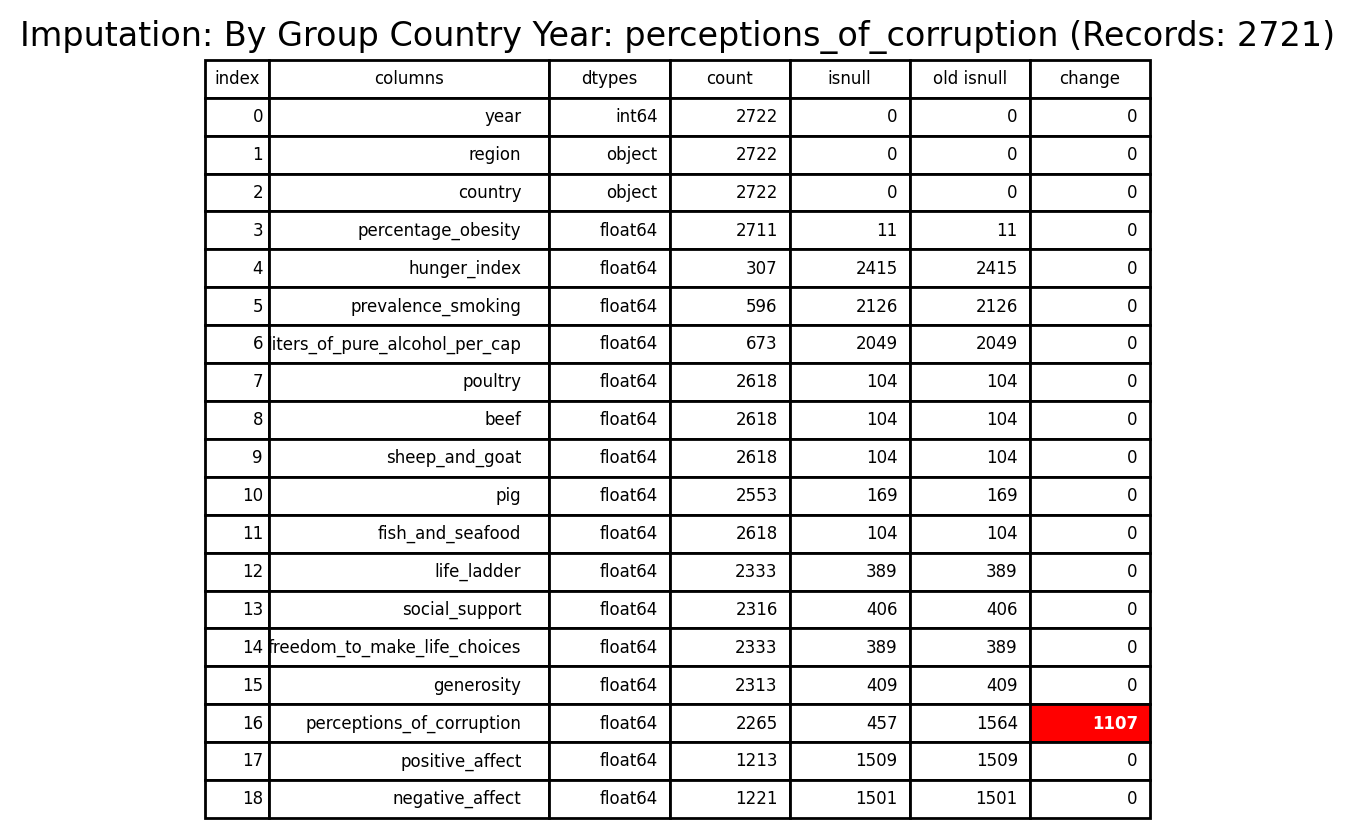
\includegraphics[scale=1]{images/dp_imputation_c_y_perceptions_of_corruption}
                        \caption{Imputation for perception\_of\_corruption grouped by country year.}
                        \label{fig:dp-impute-group-country-perception-corruption}
                \end{figure}

                \begin{figure}[H]
                        \centering
                        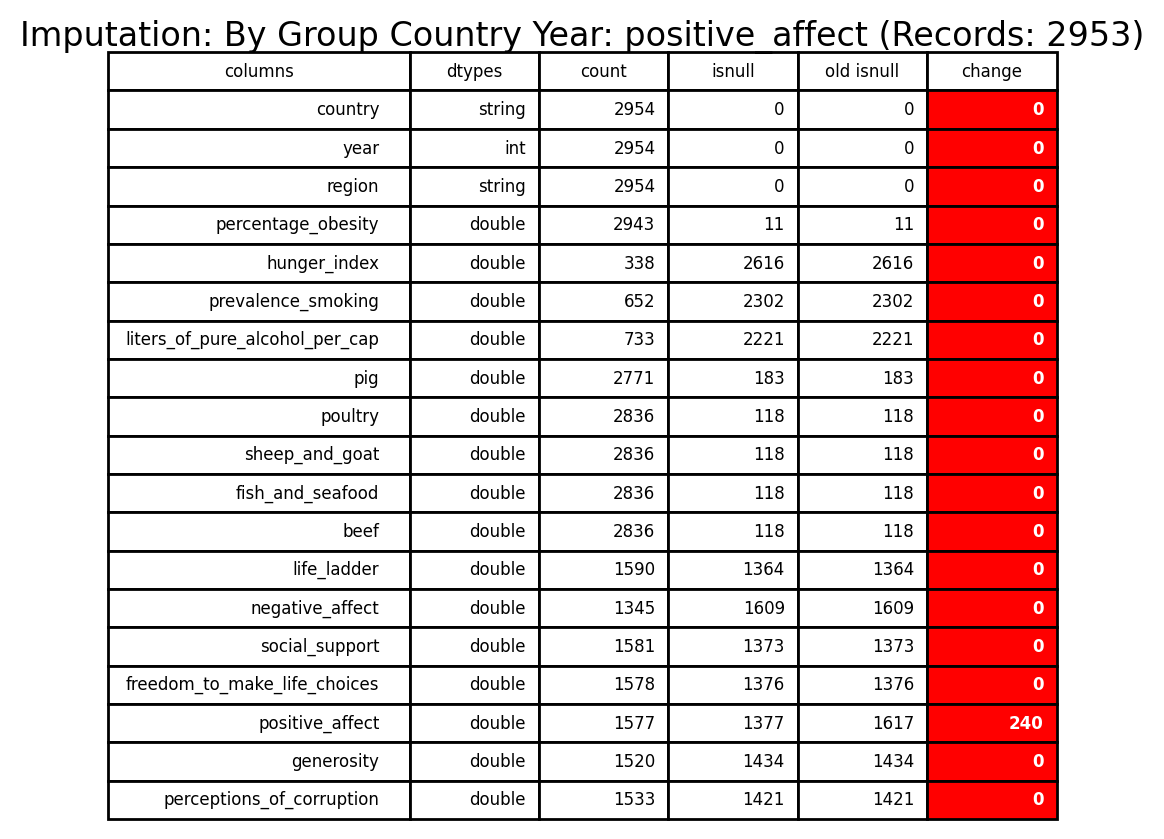
\includegraphics[scale=1]{images/dp_imputation_c_y_positive_affect}
                        \caption{Imputation for positive\_affect grouped by country year.}
                        \label{fig:dp-impute-group-country-positive-affect}
                \end{figure}

                \begin{figure}[H]
                        \centering
                        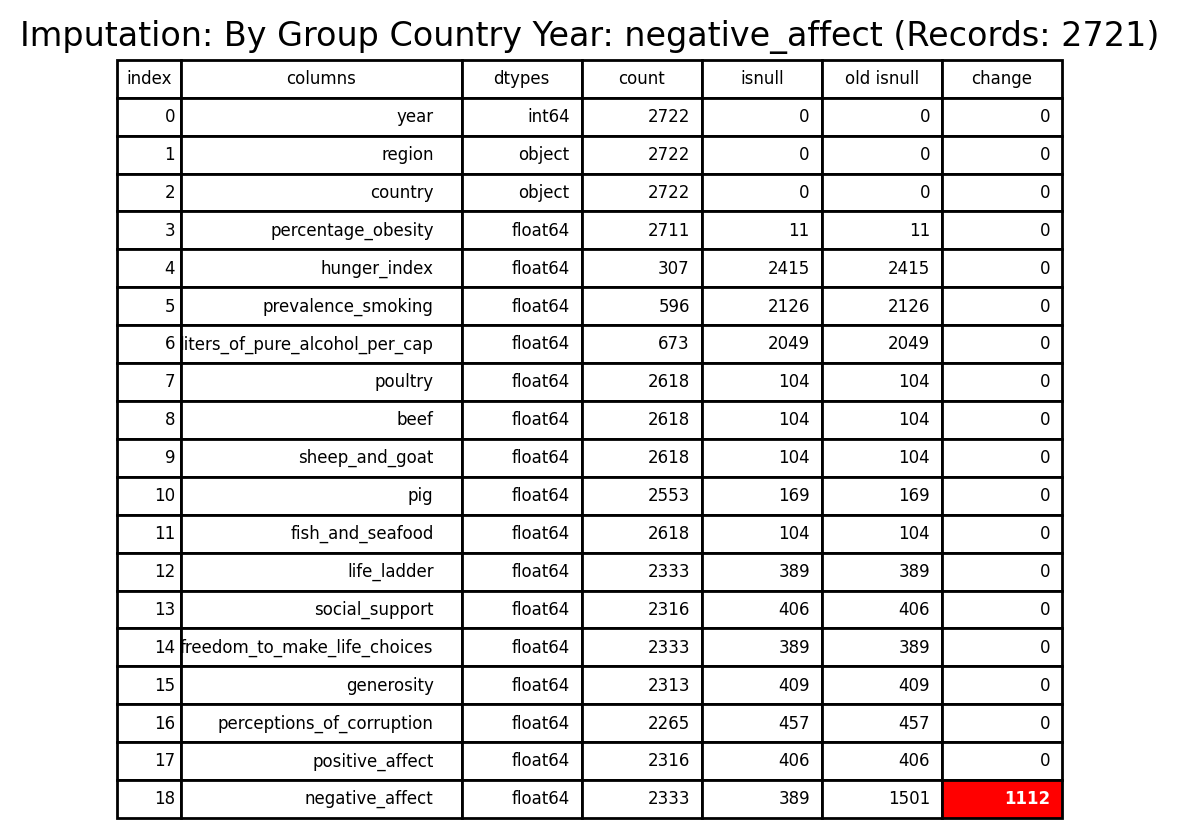
\includegraphics[scale=1]{images/dp_imputation_c_y_negative_affect}
                        \caption{Imputation for negative\_affect grouped by country year.}
                        \label{fig:dp-impute-group-country-negative-affect}
                \end{figure}

                \begin{figure}[H]
                        \centering
                        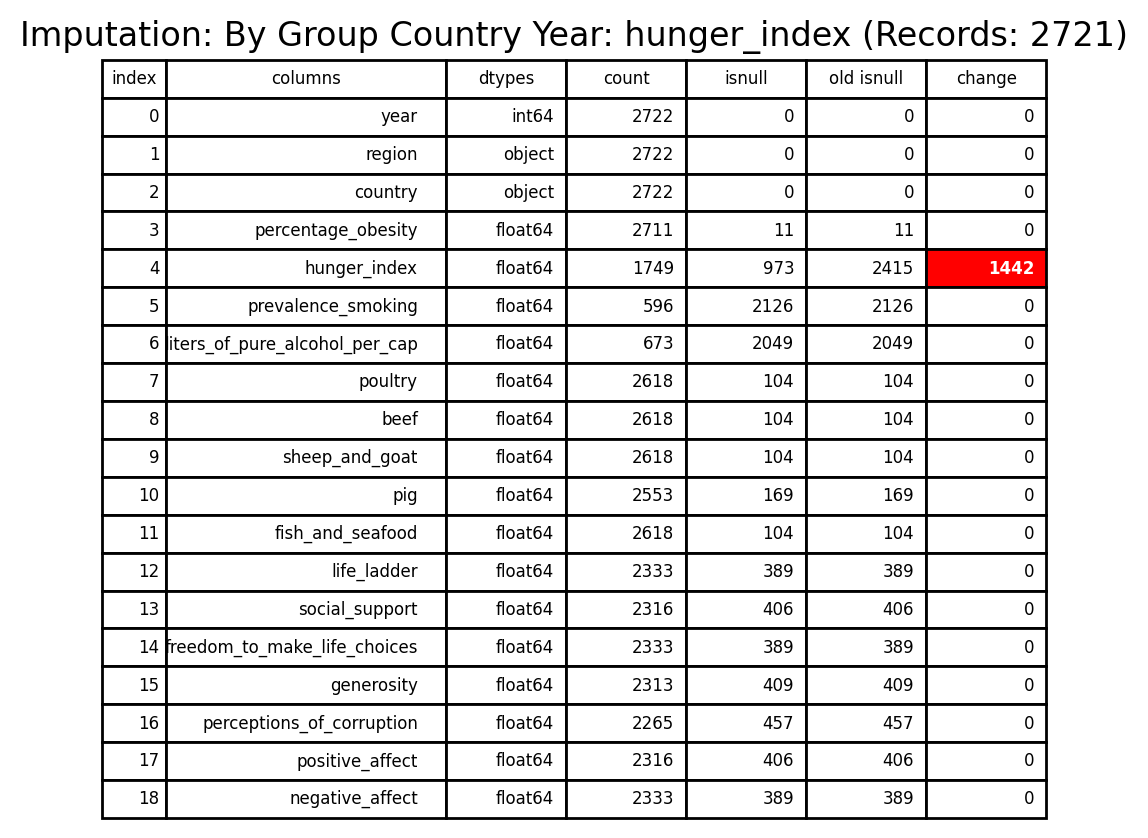
\includegraphics[scale=1]{images/dp_imputation_c_y_hunger_index}
                        \caption{Imputation for hunger\_index grouped by country year.}
                        \label{fig:dp-impute-group-country-hunger-index}
                \end{figure}

                \begin{figure}[H]
                        \centering
                        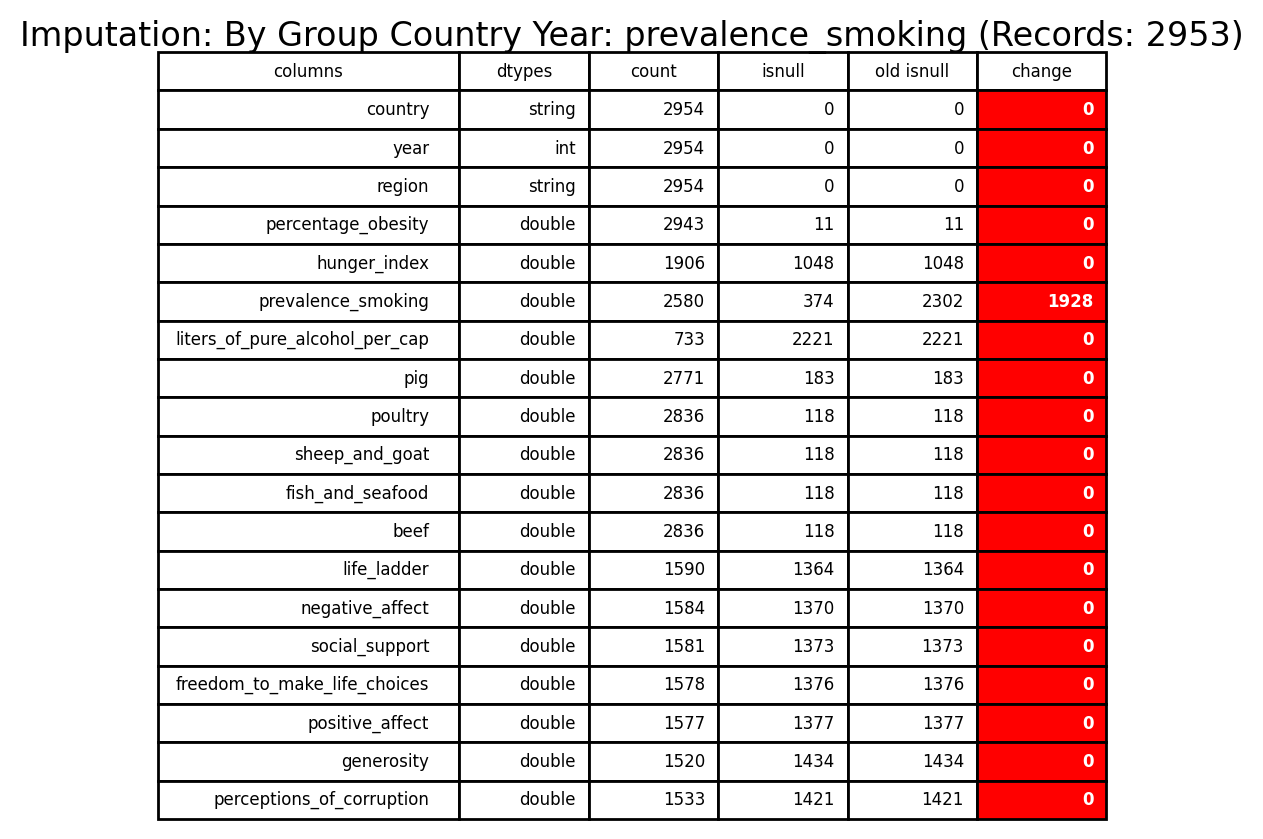
\includegraphics[scale=1]{images/dp_imputation_c_y_prevalence_smoking}
                        \caption{Imputation for prevalence\_smoking grouped by country year.}
                        \label{fig:dp-impute-group-country-prevalence-smoking}
                \end{figure}

                \begin{figure}[H]
                        \centering
                        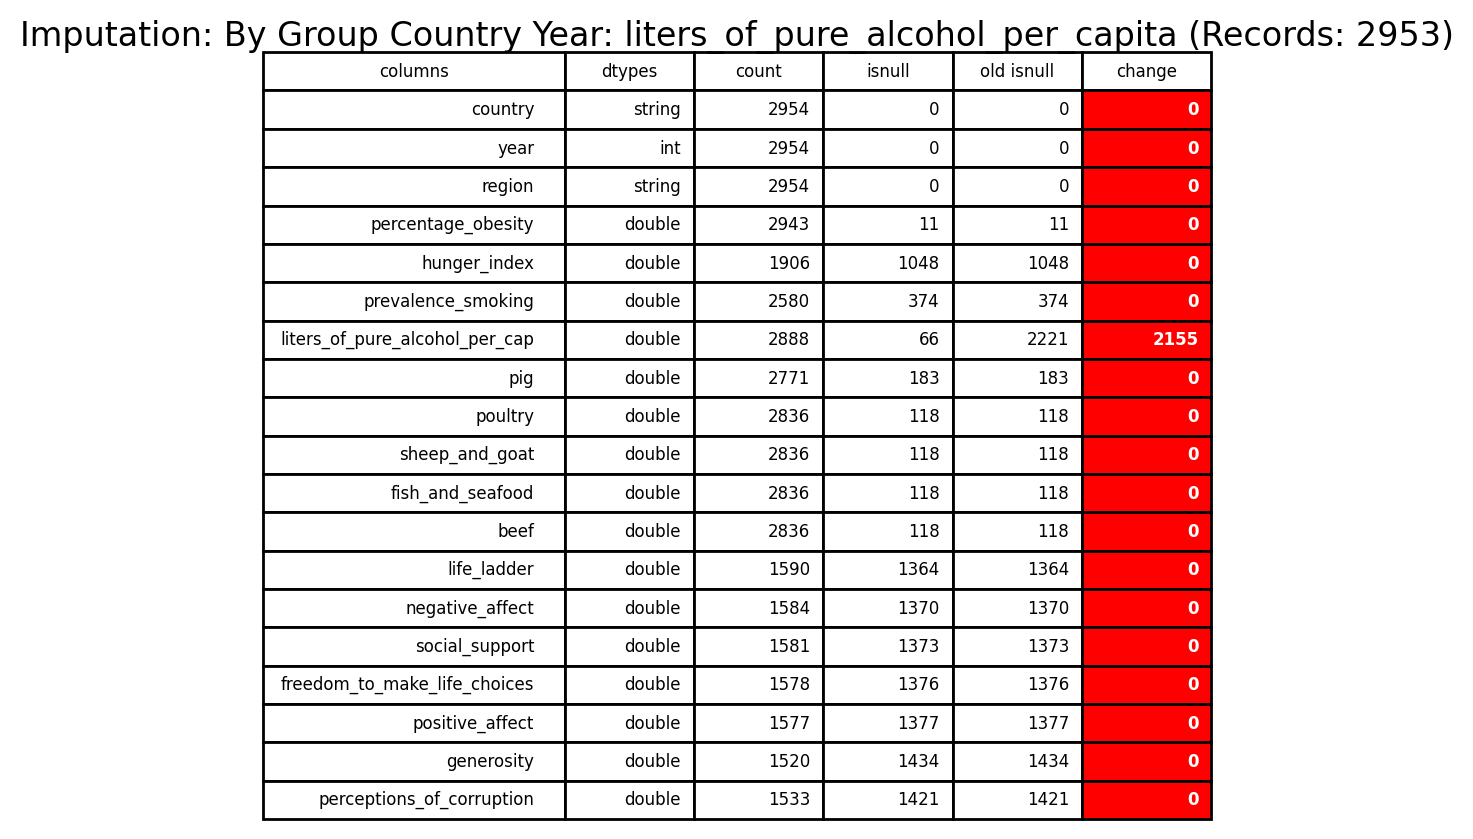
\includegraphics[scale=1]{images/dp_imputation_c_y_liters_of_pure_alcohol_per_capita}
                        \caption{Imputation for liters\_of\_pure\_alcohol\_per\_capita grouped by country year.}
                        \label{fig:dp-impute-group-country-alcohol}
                \end{figure}

                \begin{figure}[H]
                        \centering
                        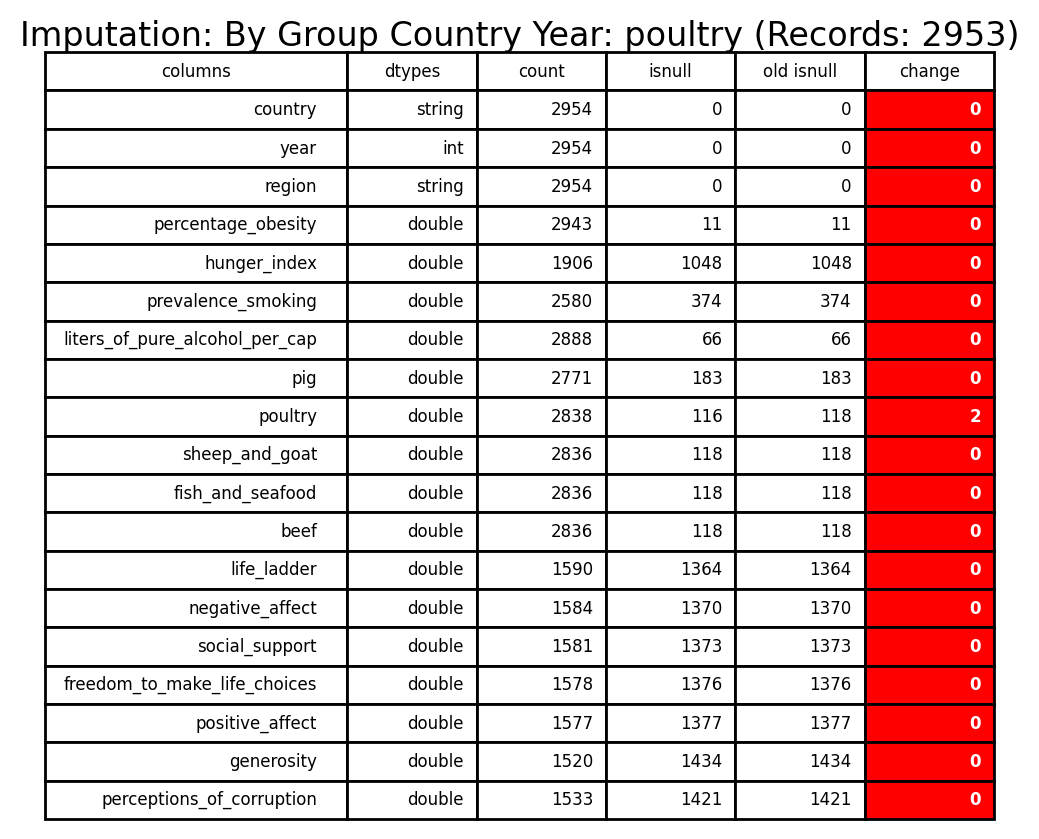
\includegraphics[scale=1]{images/dp_imputation_c_y_poultry}
                        \caption{Imputation for poultry grouped by country year.}
                        \label{fig:dp-impute-group-poultry}
                \end{figure}

                \begin{figure}[H]
                        \centering
                        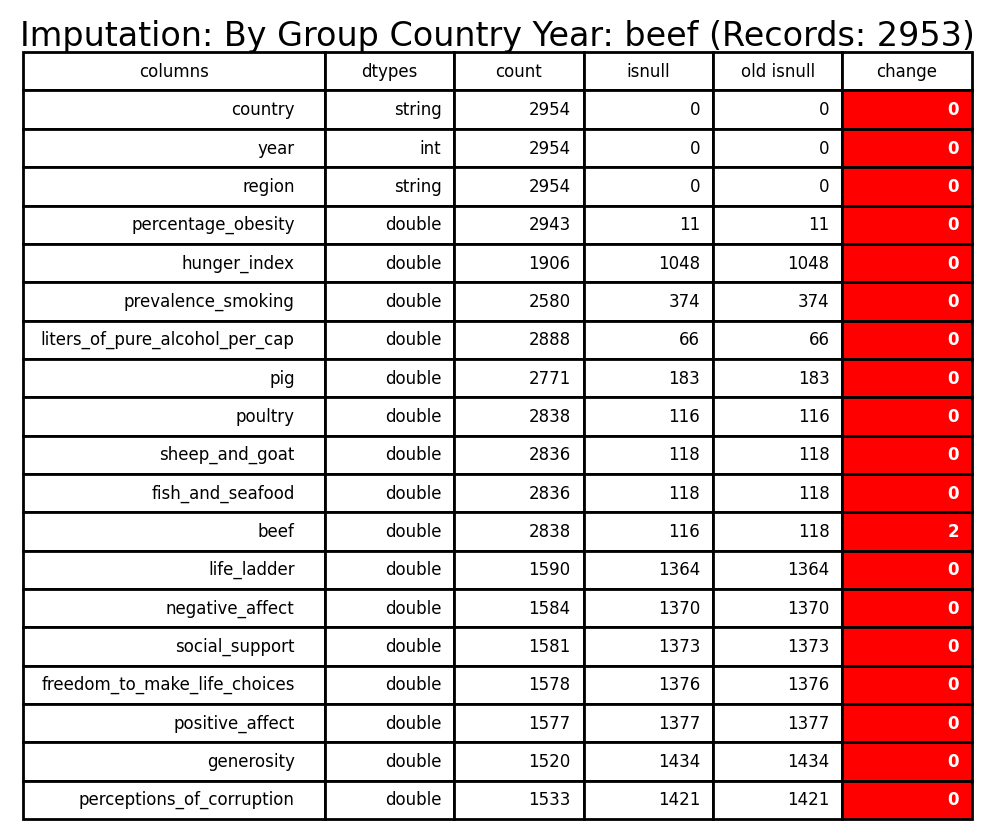
\includegraphics[scale=1]{images/dp_imputation_c_y_beef}
                        \caption{Imputation for beef grouped by country year.}
                        \label{fig:dp-impute-group-beef}
                \end{figure}

                \begin{figure}[H]
                        \centering
                        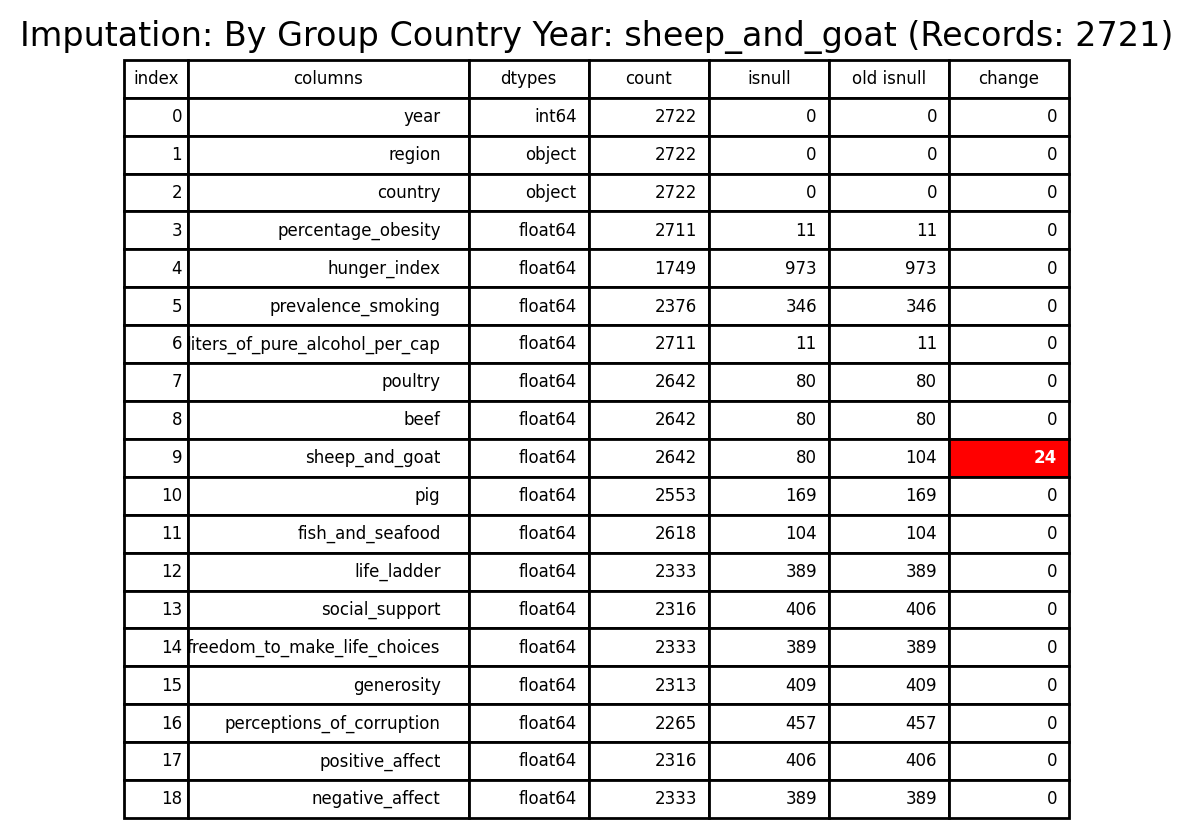
\includegraphics[scale=1]{images/dp_imputation_c_y_sheep_and_goat}
                        \caption{Imputation for sheep\_and\_goat grouped by country year.}
                        \label{fig:dp-impute-group-shep_and_goatl}
                \end{figure}

                \begin{figure}[H]
                        \centering
                        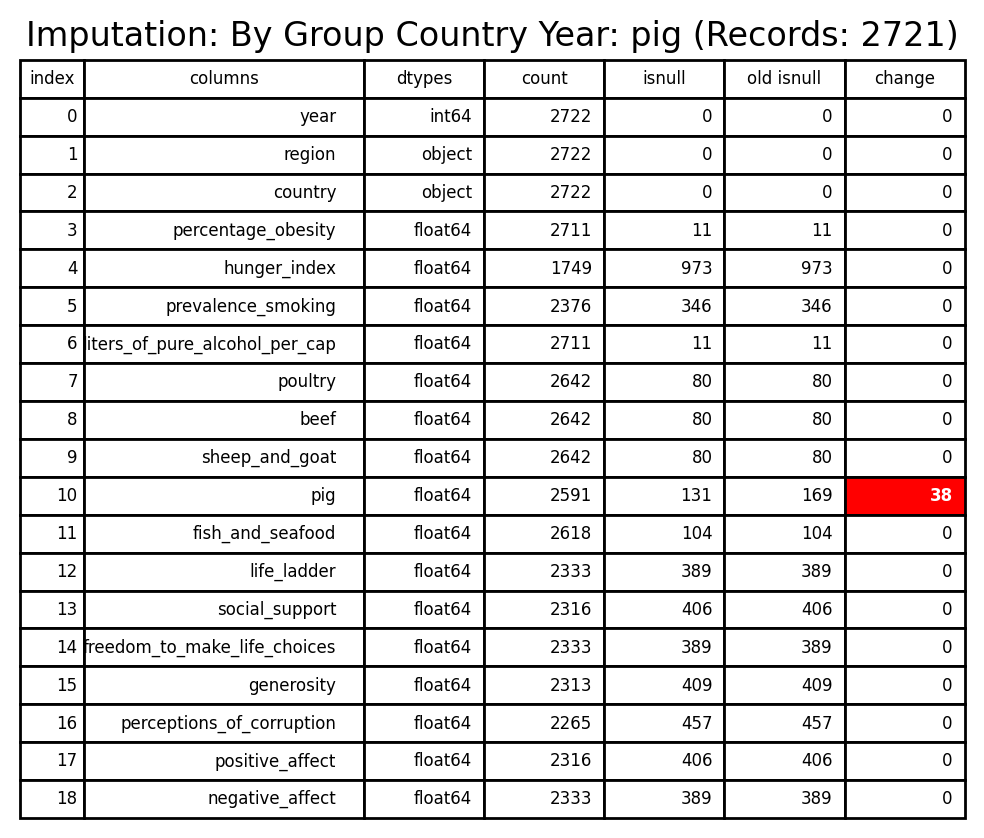
\includegraphics[scale=1]{images/dp_imputation_c_y_pig}
                        \caption{Imputation for pig grouped by country year.}
                        \label{fig:dp-impute-group-pig}
                \end{figure}

                \begin{figure}[H]
                        \centering
                        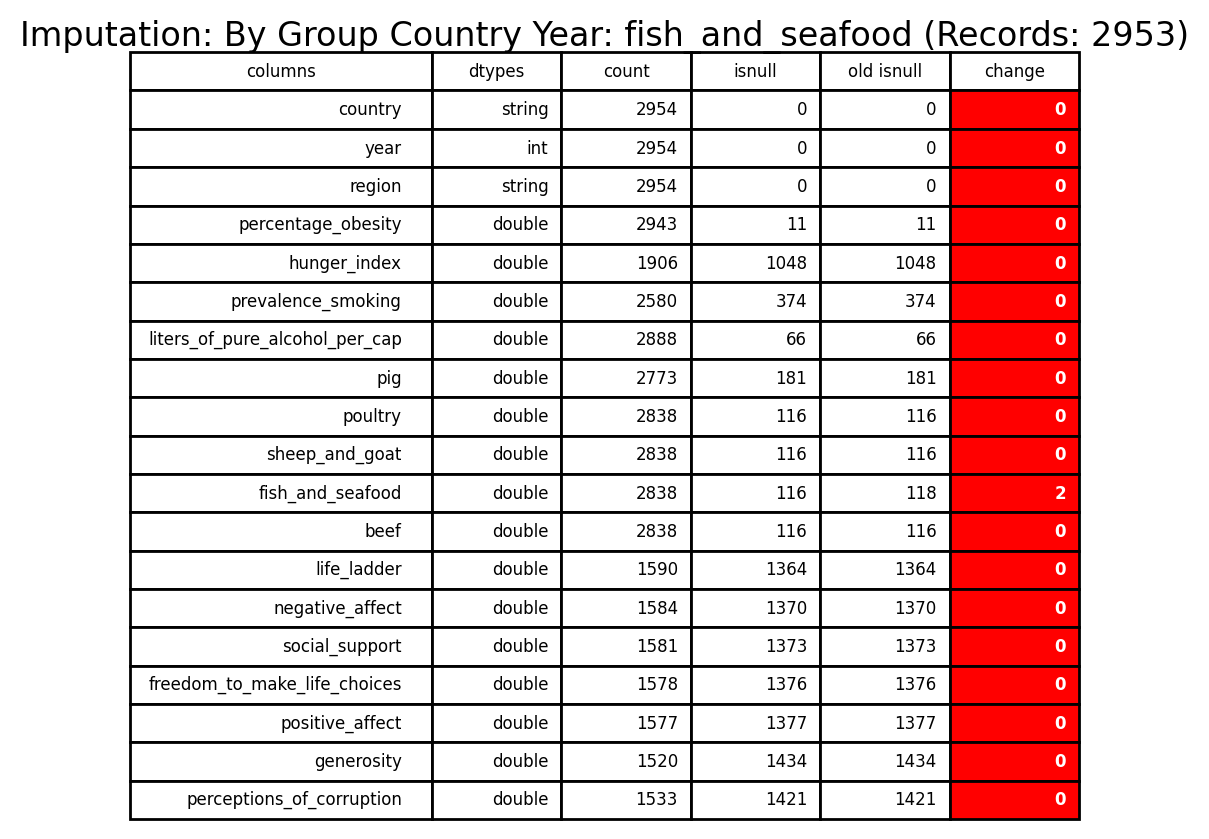
\includegraphics[scale=1]{images/dp_imputation_c_y_fish_and_seafood}
                        \caption{Imputation for fish\_and\_seafood grouped by country year.}
                        \label{fig:dp-impute-group-fish-seafood}
                \end{figure}

            \subsubsection{Imputations: By Prediction using Random Forest}
                \begin{figure}[H]
                        \centering
                        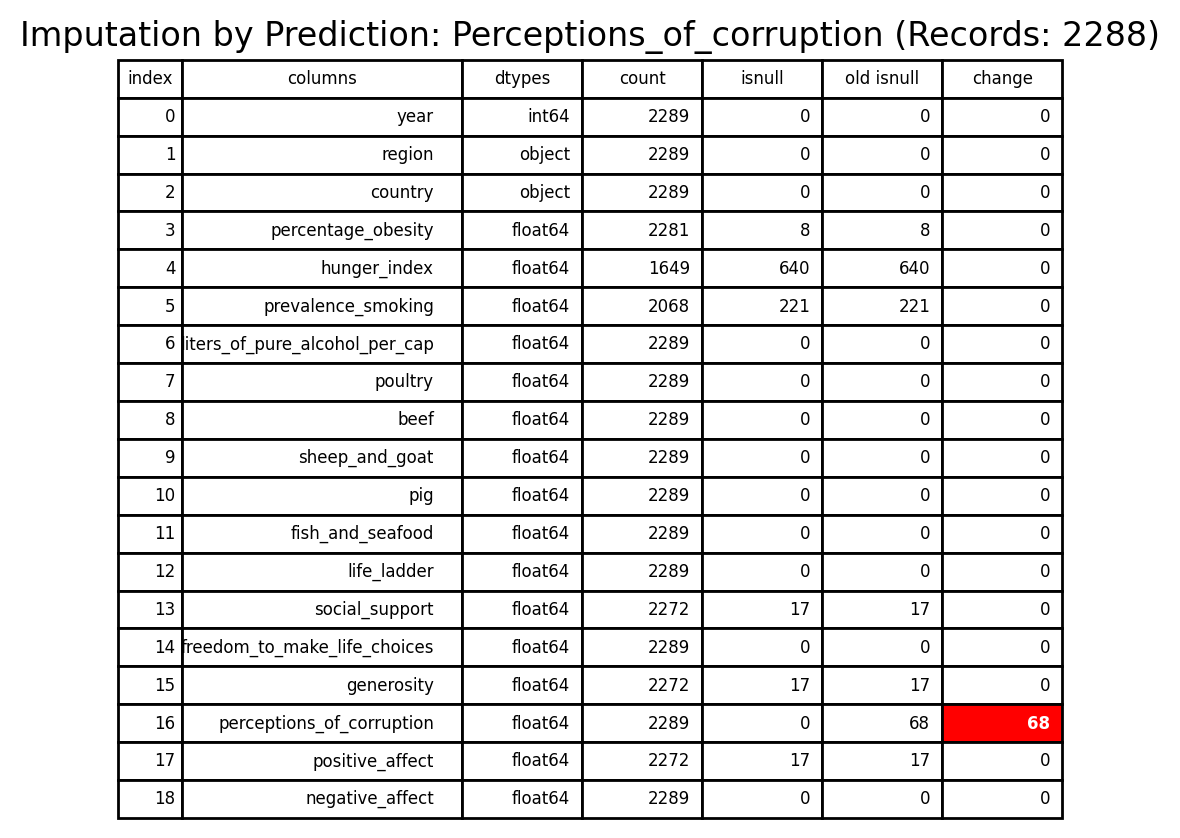
\includegraphics[scale=1]{images/dp_imput_perceptions_of_corruption}
                        \caption{Imputation for perceptions of corruption predicting with random forest.}
                        \label{fig:dp-imput-perception-corruption}
                \end{figure}
                \begin{figure}[H]
                        \centering
                        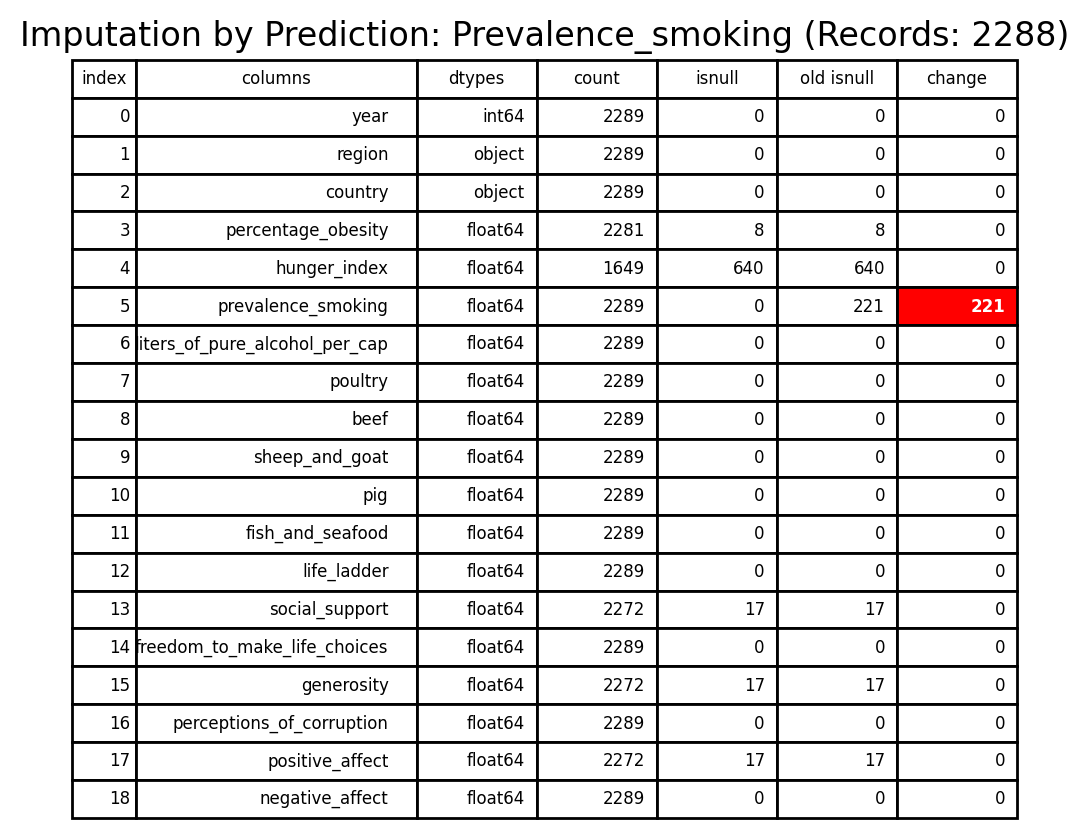
\includegraphics[scale=1]{images/dp_imput_prevalence_smoking}
                        \caption{Imputation for prevalence of smoking predicting with random forest.}
                        \label{fig:dp-imput-prevalence-of-smoking}
                \end{figure}
                \begin{figure}[H]
                        \centering
                        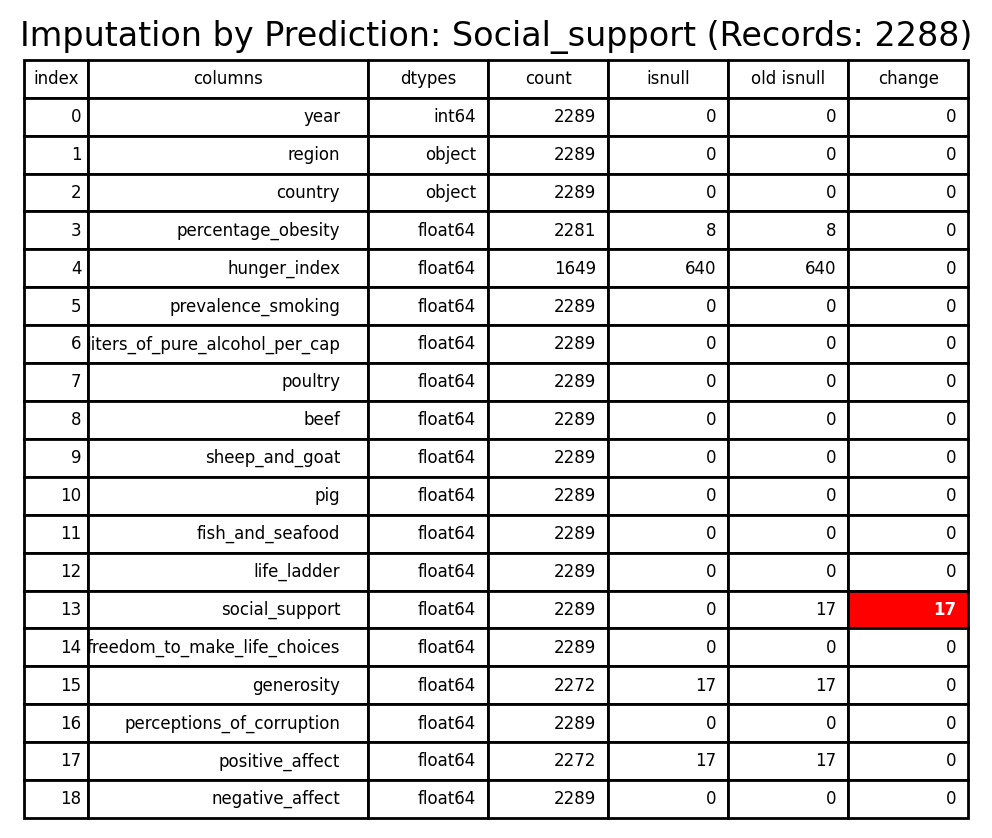
\includegraphics[scale=1]{images/dp_imput_social_support}
                        \caption{Imputation for social support predicting with random forest.}
                        \label{fig:dp-imput-social-support}
                \end{figure}
                \begin{figure}[H]
                        \centering
                        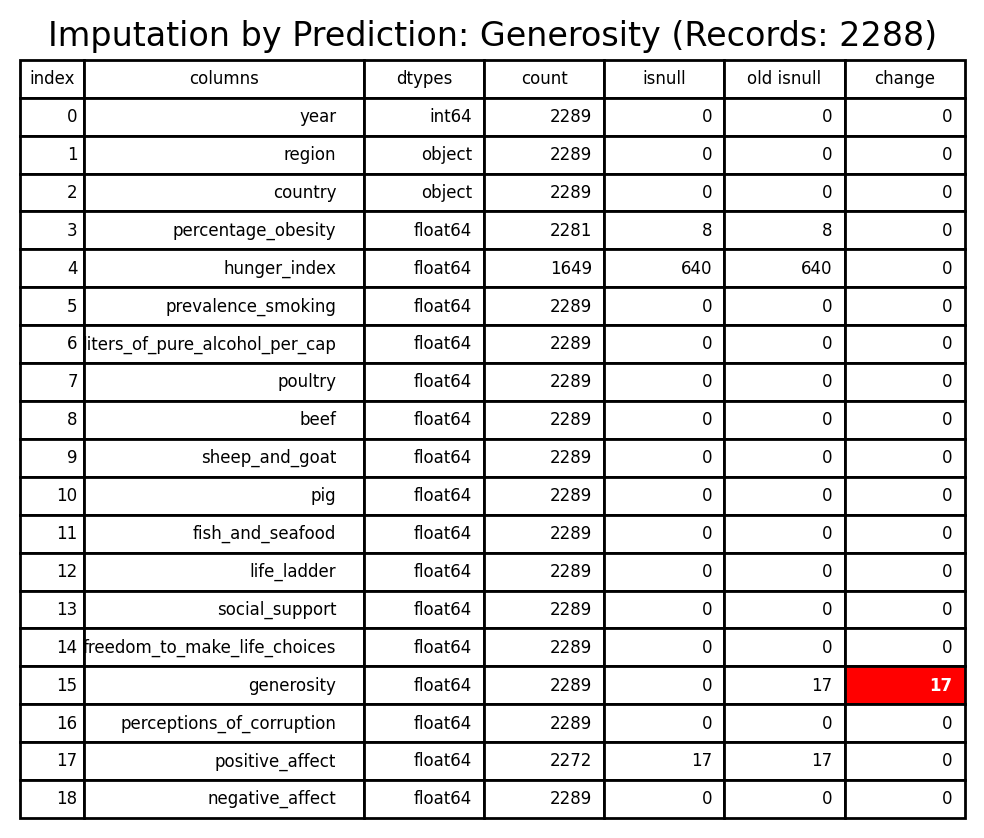
\includegraphics[scale=1]{images/dp_imput_generosity}
                        \caption{Imputation for generosity predicting with random forest.}
                        \label{fig:dp-imput-generosity}
                \end{figure}
                \begin{figure}[H]
                        \centering
                        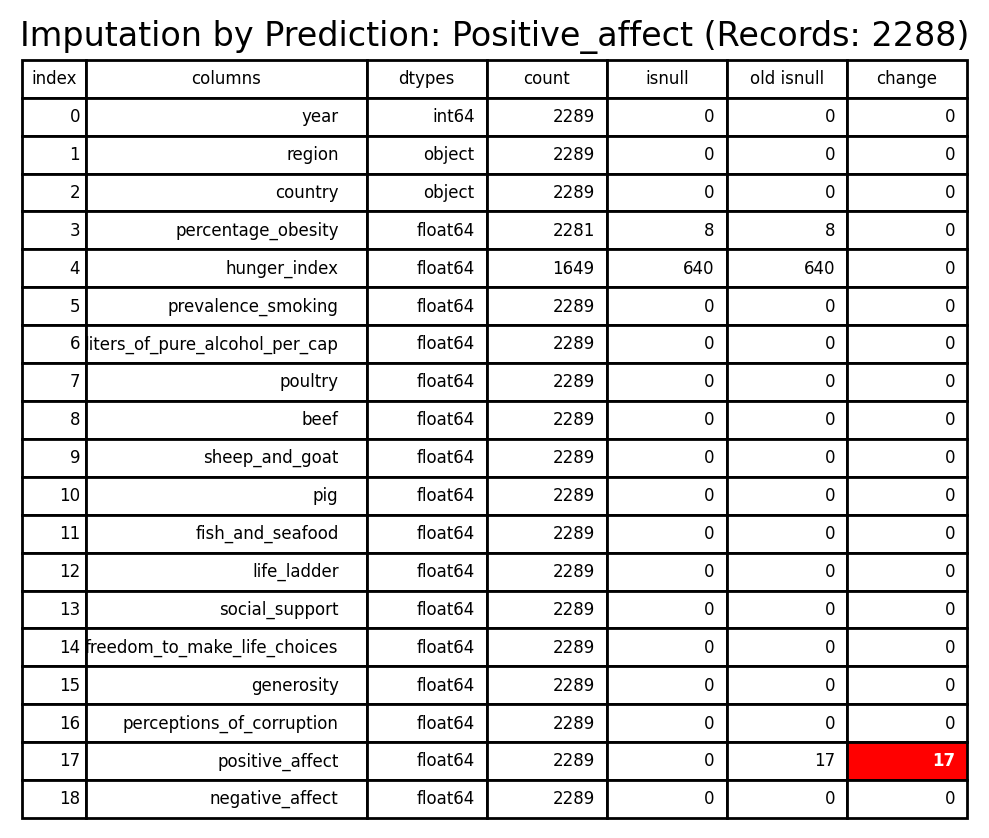
\includegraphics[scale=1]{images/dp_imput_positive_affect}
                        \caption{Imputation for positive affect predicting with random forest.}
                        \label{fig:dp-imput-positive-affect}
                \end{figure}

        \subsection{New Feature: expected\_obesity\_rate}
            A critical task performed in this phase was the creation of a new attribute named \texttt{expected\_obesity\_rate}, which acts as the target label for our predictive models. This attribute was introduced for the following reasons:

            \begin{enumerate}
                \item It allows for a more streamlined focus on the primary objective, which is to predict the expected rate of obesity in different countries.
                \item It facilitates the reduction of dimensionality by summarizing multiple features into a single, more informative attribute.
            \end{enumerate}

            The \texttt{expected\_obesity\_rate} attribute is derived based on two main criteria:

            \begin{enumerate}
                \item The percentage of obesity in a given country must be equal to or less than 20\%.
                \item The country should not be categorized as suffering from hunger.
            \end{enumerate}

            \begin{figure}[H]
                \centering
                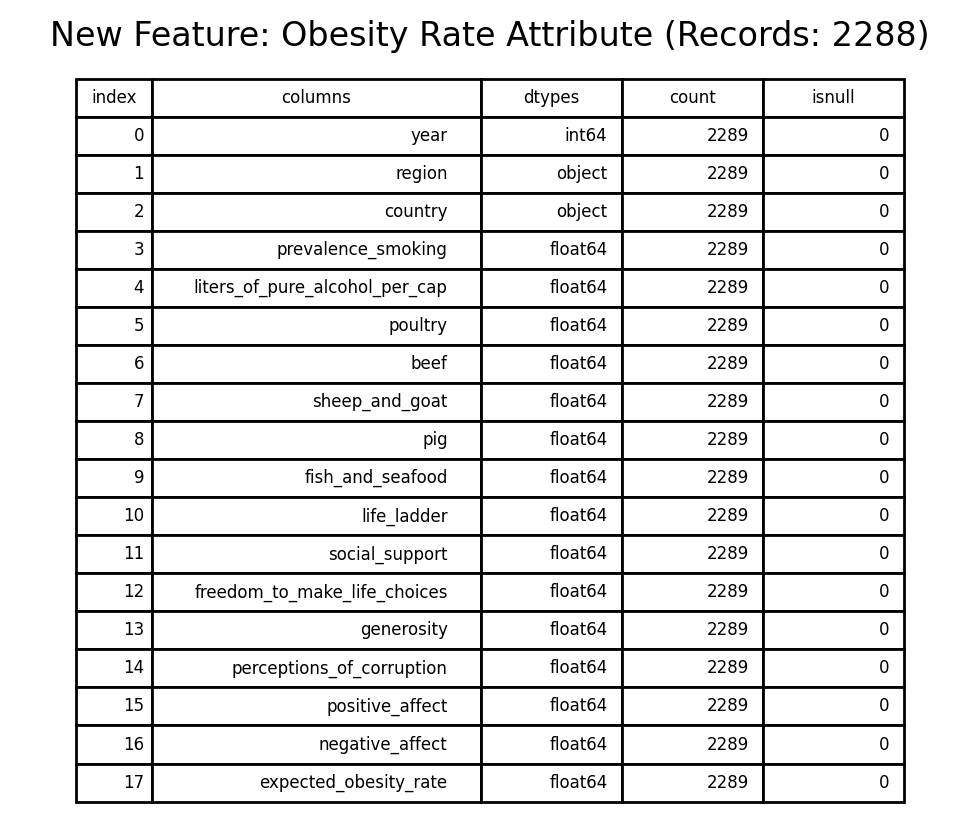
\includegraphics[scale=1]{images/dp_new_feat_obes_rate_attribute}
                \caption{New Feature expected\_obesity\_rate}
                \label{fig:dp-new-feature}
            \end{figure}


            Countries meeting both of these conditions are assigned an \texttt{expected\_obesity\_rate} value of 1; otherwise, the value is set to 0.

            As a consequence of this new attribute, the original features related to obesity percentages and hunger index were removed from the dataset. The rationale behind this action is to mitigate any risk of redundancy and to enhance the predictive power of the model by only retaining features that provide unique and meaningful insights.

            If a country meets both of these conditions, the \texttt{expected\_obesity\_rate} for that country is set to 1. Otherwise, it is set to 0.

            Upon the introduction of this new attribute, the original attributes related to obesity percentages and the hunger index were considered redundant. As such, they were removed from the dataset to prevent any potential influence on the predictive models, thereby ensuring the quality and robustness of subsequent analyses.


    \section{Where to find this phase in the code?}

        The is a file, inside the folder python, called iteration\_three.py.
        \\
        \\
        In the line 850 there is a method that execute the whole workflow.

        \begin{verbatim}
            country_manager = ProjectManager(
                generate_images_du_02=True,
            )
            country_manager.du_02()
            country_manager.du_03()
        \end{verbatim}

        All the images are being generate by code and referenced by using LatEx to create this document.